\begin{frame}{Experiment 1}
\setbeamercovered{invisible}
\fontsize{12pt}{15}\selectfont
\vspace{-0.5cm}
{\Large\textbf{Results:}}\\
\vspace{0.2cm}

\only<1>{\begin{figure}
    \centering
    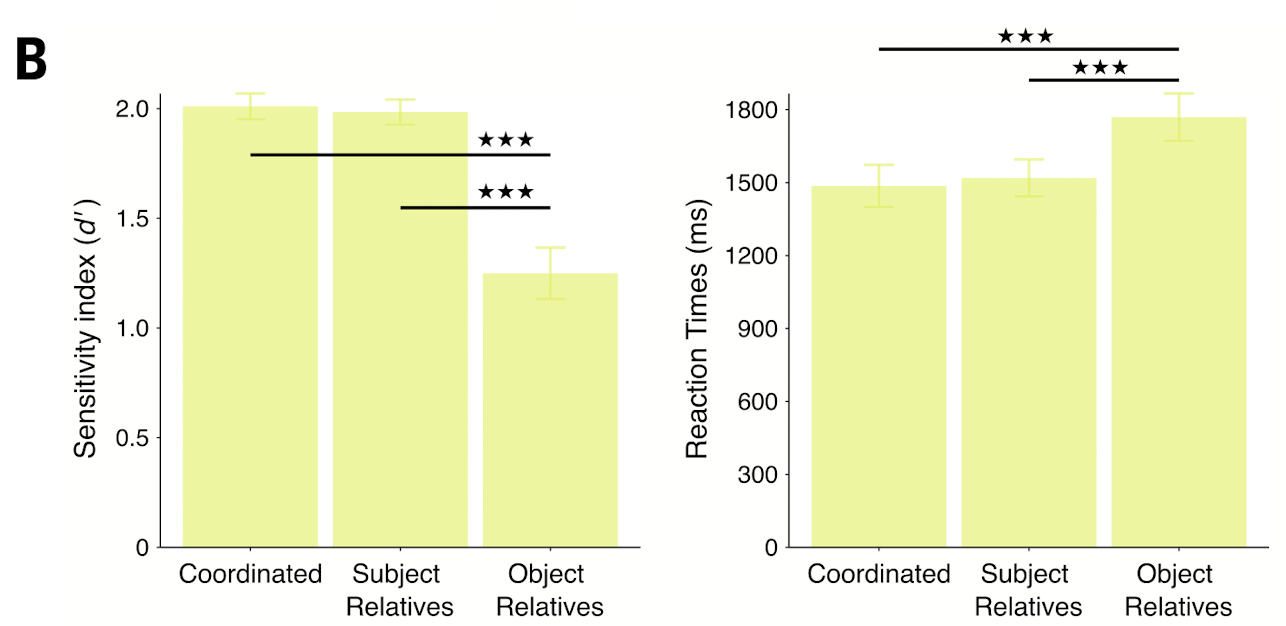
\includegraphics[width=8cm]{images/paper_pics/fig1B.png}
    \caption*{Object-relative clauses show worst sensitivity index scores and longest reaction time}
    \label{fig:label2}
\end{figure}}
\pause

\only<2>{\begin{itemize}\item \textbf{No difference} between subject-relative and coordinated clauses
\item $\rightarrow$ \textbf{Syntactic complexity} of the object relatives
\end{itemize}}
\pause
\only<3>{\begin{itemize} 
\item They assessed functional syntactic network by contrasting brain activation during object relatives vs the two other types of clauses.
\item Syntactic network: parietofrontal ensemble and BG (caudate nuclei, GPi, putamen). Left IFG also.
\end{itemize}}


\end{frame}